\section{Results and Analysis}
\label{sec:results}

\subsection{Main Benchmark Comparison}

The final CodeGraph configuration achieves \textbf{74.0\% Recall@10}, an absolute improvement of 24.3 percentage points over the strong BM25-only baseline. \Cref{tab:main-results} presents the final comparative evaluation. Because the retrieval pipeline relies on deterministic algorithms (static parsing, BM25 matching, and exact PageRank calculation), these results are stable and not subject to the statistical variance that affects LLM-mediated retrieval loops.

\begin{table}[htbp]
    \centering
    \caption{Main quantitative comparison on SWE-bench Lite (300 instances).}
    \label{tab:main-results}
    \begin{adjustbox}{max width=\linewidth}
    \begin{tabularx}{\linewidth}{@{} >{\RaggedRight\arraybackslash}X >{\RaggedRight\arraybackslash}p{1.2cm} >{\RaggedRight\arraybackslash}p{1.2cm} >{\RaggedRight\arraybackslash}p{1.2cm} >{\RaggedRight\arraybackslash}p{1.6cm} @{}}
        \toprule
        \textbf{Method} & \textbf{R@5} & \textbf{R@10} & \textbf{MRR} & \textbf{Zero-recall} \\
        \midrule
        BM25-only Baseline & 37.7\% & 49.7\% & 0.248 & 151 \\
        CodeGraph (Initial) & 37.0\% & 42.0\% & 0.228 & 174 \\
        \textbf{CodeGraph (Final)} & \textbf{60.7\%} & \textbf{74.0\%} & \textbf{0.442} & \textbf{78} \\
        \bottomrule
    \end{tabularx}
    \end{adjustbox}
\end{table}

\subsection{Engineering Trajectory and Ablation}

The initial configuration of CodeGraph (42.0\% R@10) underperformed the lexical baseline. The final result (74.0\% R@10) was reached through systematic refinement of the seed stage (\Cref{fig:trajectory}).

\begin{figure}[htbp]
    \centering
    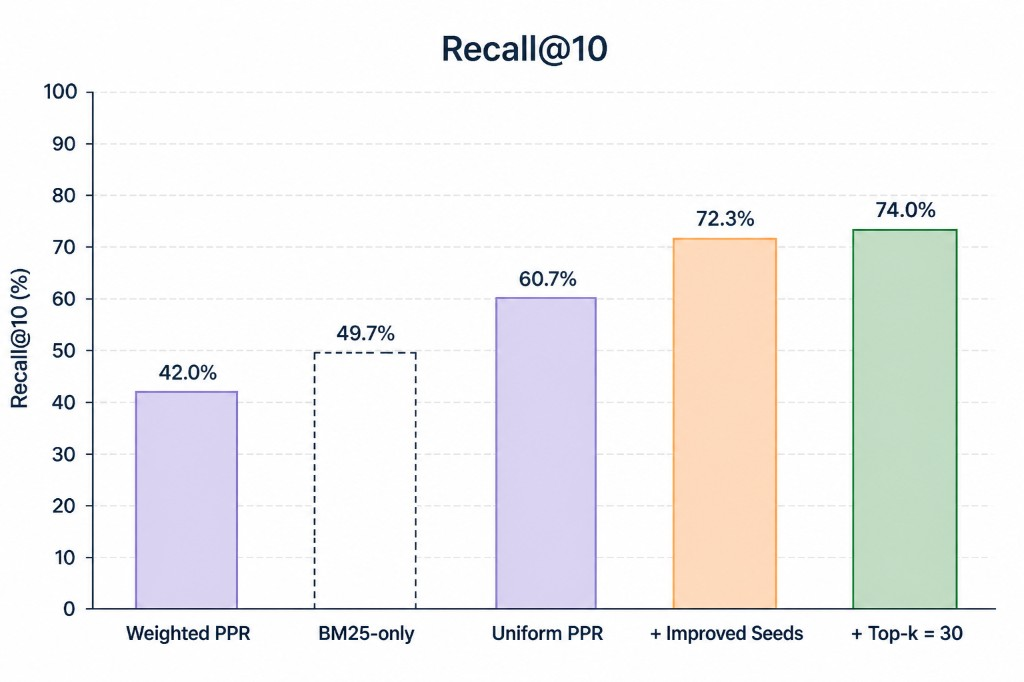
\includegraphics[width=\linewidth]{assets/recall_trajectory.png}
    \caption{Recall@10 engineering trajectory. Successive algorithmic and lexical refinements recovered the initial performance deficit and surpassed the lexical baseline.}
    \label{fig:trajectory}
\end{figure}

The improvement breaks down into three sequential interventions:
\begin{enumerate}
    \item \textbf{Algorithm Refinement (+18.7pp):} Switching from confidence-weighted to uniform PPR restart closed the gap with BM25. When seeds are noisy, assigning them proportional weights amplifies false positives. Uniform restart allows the graph topology itself to arbitrate relevance through path convergence.
    \item \textbf{Seed Engineering (+11.6pp):} Implementing compound tokenization, an expanded BM25 corpus, and IDF entity weighting ensured that task descriptions resolved to structurally meaningful starting nodes.
    \item \textbf{Budget Adjustment (+1.7pp):} Increasing the output threshold from 20 to 30 files recovered instances where the target was correctly identified but ranked just outside the initial cutoff.
\end{enumerate}

To test the schema's reliance on explicit dependencies, we conducted an ablation that augmented the graph with \texttt{CO\_LOCATED} proximity edges between sibling files. This caused a 1.0pp regression: artificial density dilutes relevance across unrelated files, proving that CodeGraph's precision derives strictly from high-fidelity dependency links rather than structural heuristics.

\subsection{The Reachability Bottleneck}

A defining characteristic of CodeGraph is its bimodal rank distribution: the target file almost always lands in the top-5 or does not appear in the top-10 at all. As \Cref{fig:bimodal} shows for the initial configuration, only 5\% of instances fell into the intermediate band (ranks 6--10).

\begin{figure}[htbp]
    \centering
    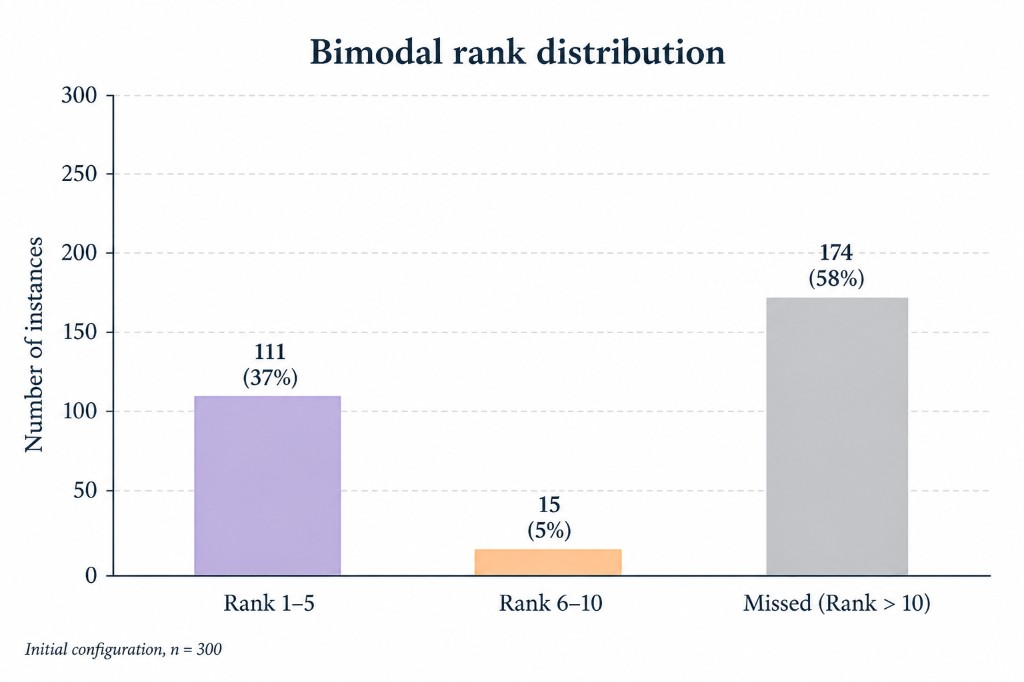
\includegraphics[width=\linewidth]{assets/bimodal_rank_distribution.png}
    \caption{Bimodal rank distribution for the initial configuration. The near-absence of intermediate ranks indicates that Reachability is the primary bottleneck.}
    \label{fig:bimodal}
\end{figure}

This pattern yields our central empirical finding: the retrieval ceiling is bounded by Reachability, not Ranking. If the system retrieves the target file at all, the PPR algorithm ranks it highly. The zero-recall failures occur exclusively when no seed lies on a structurally connected path to the target. When seeds miss the relevant neighbourhood entirely, the graph has no signal to propagate. This diagnostic directly motivated our emphasis on seed quality engineering rather than advanced ranking heuristics.

\subsection{Qualitative Retrieval Cases}

To illustrate how the hybrid mechanism operates in practice, we examine two representative retrieval episodes: one success and one failure.

\textbf{Success Case (Structural Amplification):} In \textit{matplotlib/matplotlib-23562}, the bug report requests support for a new 3D surface attribute. The issue text briefly mentions \texttt{Poly3DCollection}. The lexical index correctly identifies \texttt{Poly3DCollection} as a seed, but it also falsely matches generic terms like \texttt{color} and \texttt{facecolors} across dozens of unrelated files. During structural propagation, the generic seeds dissipate their probability mass across disparate, disconnected utility modules. Conversely, the specific seed \texttt{Poly3DCollection} propagates its mass locally through direct \texttt{CALLS} and \texttt{INHERITS\_FROM} edges. The target file, \texttt{lib/mpl\_toolkits/mplot3d/art3d.py}, absorbs this concentrated mass and is ranked at position 1. This demonstrates graph topology successfully filtering out lexical noise.

\textbf{Failure Case (Semantic Gap):} In \textit{django/django-11001}, the user describes a bug where ``raw SQL queries containing multi-line strings cause a syntax error.'' The description is entirely conceptual and uses no actual Django source-code identifiers. Because the words ``raw'', ``SQL'', and ``syntax'' do not uniquely match the specific compiler classes responsible for the bug (e.g., \texttt{SQLCompiler} in \texttt{django/db/models/sql/compiler.py}), the lexical stage fails to extract any meaningful seeds. Without a localized entry point, PPR cannot traverse the relevant dependency subgraph, resulting in a zero-recall failure. This case perfectly illustrates the structural ceiling: no amount of sophisticated graph routing can compensate for a total failure to enter the correct structural neighbourhood.
